\documentclass[a4paper,12pt]{report}

\usepackage[utf8]{inputenc} 
\usepackage[margin=2cm]{geometry}  
\usepackage[brazilian]{babel} 
\usepackage{multirow}
\usepackage{graphicx}
\usepackage{caption}
\usepackage{subcaption}
\usepackage{mwe}
\usepackage{textcomp} %Impede erros do gensymb
\usepackage{gensymb} %Degree º symbol
\usepackage{pdflscape} %landscape pages
\usepackage{pdfpages} %For including PDFs with \includepdf
\usepackage{amsmath}
\usepackage{verbatim}
\usepackage{amssymb}
\usepackage{setspace}
\usepackage{mathtools}
\usepackage{hyperref}
\usepackage{tikz}
\usepackage{float}  
\pagenumbering{arabic}

\usepackage{indentfirst} %\section or \chapter by default don't indent the first paragraph for some absurd reason!


%\singlespacing Para um espaçamento simples
%\onehalfspacing Para um espaçamento de 1,5
%\doublespacing Para um espaçamento duplo

\graphicspath{{images/}}


\begin{document}
	
	\begin{titlepage}
		\begin{center}
			
			\Large
			UNIVERSIDADE FEDERAL DE SANTA CATARINA\\
			EEL7051 - Materiais Elétricos\\
			\vspace*{5cm}
			\Huge
			\textbf{PROJETO PRÁTICO DE MATERIAIS ELÉTRICOS}\\
			\textbf{TERMOPARES:}\\
			\textbf{Princípios, construção, normas e aspectos práticos}
			
			\vspace{1.5cm}
			
			\vfill
			\Large
			\textbf{Alunos: Bobão 1}\\
			\textbf{Alunos: Bobão 2}\\
			\textbf{Alunos: Bobão 3}\\
			
			\textbf{Professor: Rambo} %Inserir nome completo do Rambo
			\vspace{0.8cm}
			
			Departamento de Engenharia Elétrica e Eletrônica\\
			Curso de Graduação em Engenharia Eletrônica\\
			Brasil\\
			
			
			
		\end{center}
	\end{titlepage}
	\Large
	
	\pagebreak
	\listoffigures
    \pagebreak
    \tableofcontents
	
	\chapter{Introdução Teórica}
	
	Termopares são dispositivos formados pela junção de dois materiais condutores ou, por vezes, semicondutores, distintos, unidos em uma extremidade e sensíveis à variação de temperatura, expressando esta sensibilidade através de uma diferença de potencial. Possuem larga utilização industrial e em sistemas de instrumentação para aferição de temperatura, sendo o mais conhecido método para este tipo de medição.
	
	\noindent Um termopar é também conhecido por sua versatilidade como sensor de temperatura, portanto, normalmente são utilizados em uma ampla gama de aplicações - desde um termopar de uso industrial à um termopar regularmente encontrado em utilitários e aparelhos regulares. Devido à sua vasta gama de modelos e especificações técnicas, é extremamente importante entender a sua estrutura básica, como um termopar funciona, suas escalas para melhor determinar qual é o tipo certo e material do termopar para sua aplicação.
	
	\begin{figure}[htbp]
		\centering
		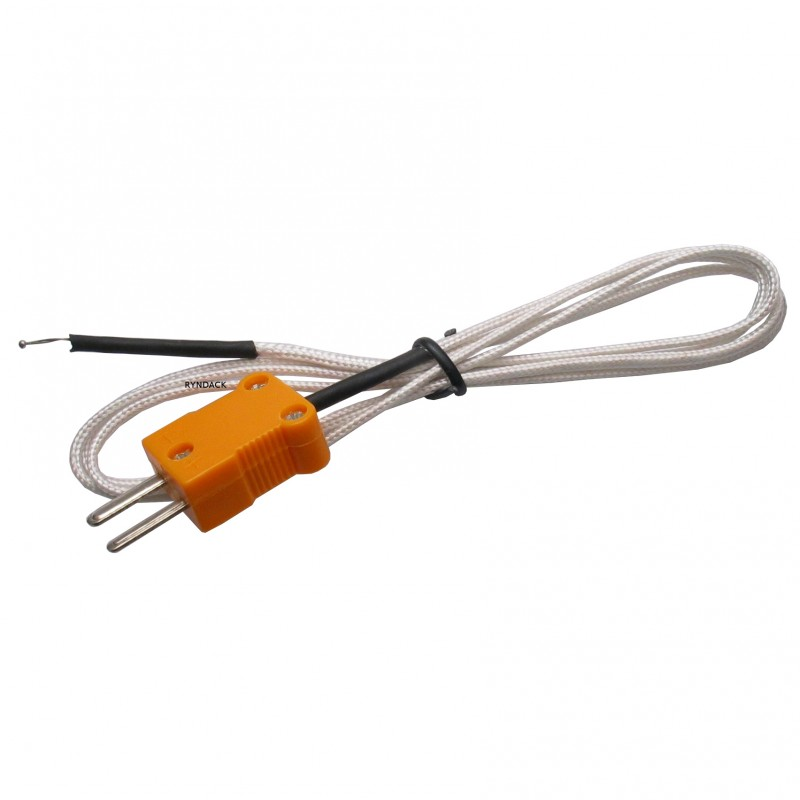
\includegraphics[scale=.2]{termopar-tipo-k-01.jpg}
		\caption{Termopar Tipo K}
		\label{real}
	\end{figure}
	
	\chapter{Princípios físicos}
	Ao ser aplicada uma diferença de temperatura entre a junção de metais e as extremidades livres, haverá a geração de uma diferença de potencial da ordem de mV (milivolts) entre estas extremidades, da qual pode ser medida por um sistema de aquisição, utilizando-se comumente um multímetro como pode ser observado no esquemático da Figura \ref{esquematico}.
	
	\hfill \break
	\hfill \break
	
	\begin{figure}[htbp]
		\centering
		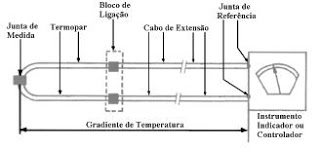
\includegraphics[]{ABAAAAJ_sAG-68.jpg}
		\caption{Utilização do Termopar tipo K}
		\label{esquematico}
	\end{figure}
	
	\pagebreak
	
	\section{Efeito Seebeck}
	
	O princípio termoelétrico dos termopares deriva de uma propriedade física dos condutores metálicos, que quando  submetidos a um gradiente térmico em suas extremidades: a extremidade mais quente faz com que os elétrons dessa região tenham maior energia cinética e se acumulem no lado mais frio, gerando uma diferença de potencial elétrico entre as extremidades do condutor na ordem de alguns milivolts, como está representado na Figura \ref{seebeck}.
	
	\begin{figure}[htbp]
		\centering
		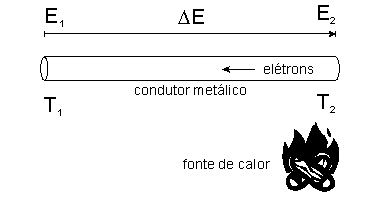
\includegraphics[scale=.8]{PrincipioTermoeletrico1.jpg}
		\caption{Efeito Seebeck}
		\label{seebeck}
	\end{figure}
	
	\noindent Podemos relacionar a temperatura com a força eletromotriz $\Delta E$ medido pelo coeficiente termodinâmico de Seebeck, representado na Equação \ref{seeback_eq}.
	
	\begin{equation}
	S = \frac{\Delta E}{\Delta T}
	\label{seeback_eq}
	\end{equation}  
	
	\noindent Quando dois condutores metálicos de natureza diferente são acoplados, na presença um gradiente de temperatura, os elétrons de um metal tendem a migrar de um condutor para outro, gerando uma diferença de potencial entre suas extremidades livres, como representado na Figura \ref{seebeck2}, de acordo com com seus coeficientes $S$, temos que a diferença de potencia gerada por essa diferença segue a Equação \ref{seeback_eq2}.
	
	\begin{figure}[htbp]
		\centering
		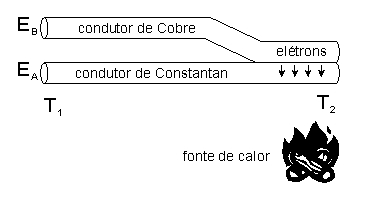
\includegraphics[scale=.8]{PrincipioTermoeletrico2.jpg}
		\caption{Efeito Seebeck para dois condutores diferentes}
		\label{seebeck2}
	\end{figure}
	
	\begin{equation}
	E = \int_{T_{1}}^{T_{2}} (S_{B}(T) - S_{A}(T))~\mathrm{d}T
	\label{seeback_eq2}
	\end{equation}
	
	\noindent Aproximando linearmente, para uma região de temperatura  onde os coeficientes possam ser considerados contantes podemos chegar na seguinte simplificação.
	
	\begin{equation}
	E = (S_{B} - S_{A}) \cdot  (T_{2} - T_{1})
	\end{equation}
	
	\noindent Podemos inclusive aplicando a equação \ref{densidade}, para assim determinar densidade termoelétrica do material.
	
	\begin{equation}
	J = \sigma (-\Delta V + E)
	\label{densidade}
	\end{equation}
	
	\noindent Onde $J$ é a densidade termoelétrica do material e $\sigma$ a condutividade do meio.
	
	\subsection{Efeito Peltier}
	O efeito Peltier se comporta de forma inversa ao efeito Seebeck, pois este efeito consiste consiste na produção de um gradiente de temperatura na junção de dois condutores de materiais diferentes quando submetidos a uma tensão elétrica em circuito fechado, como pode ser observado na Figura \ref{peltier} . 
	
	\begin{figure}[htbp]
		\centering
		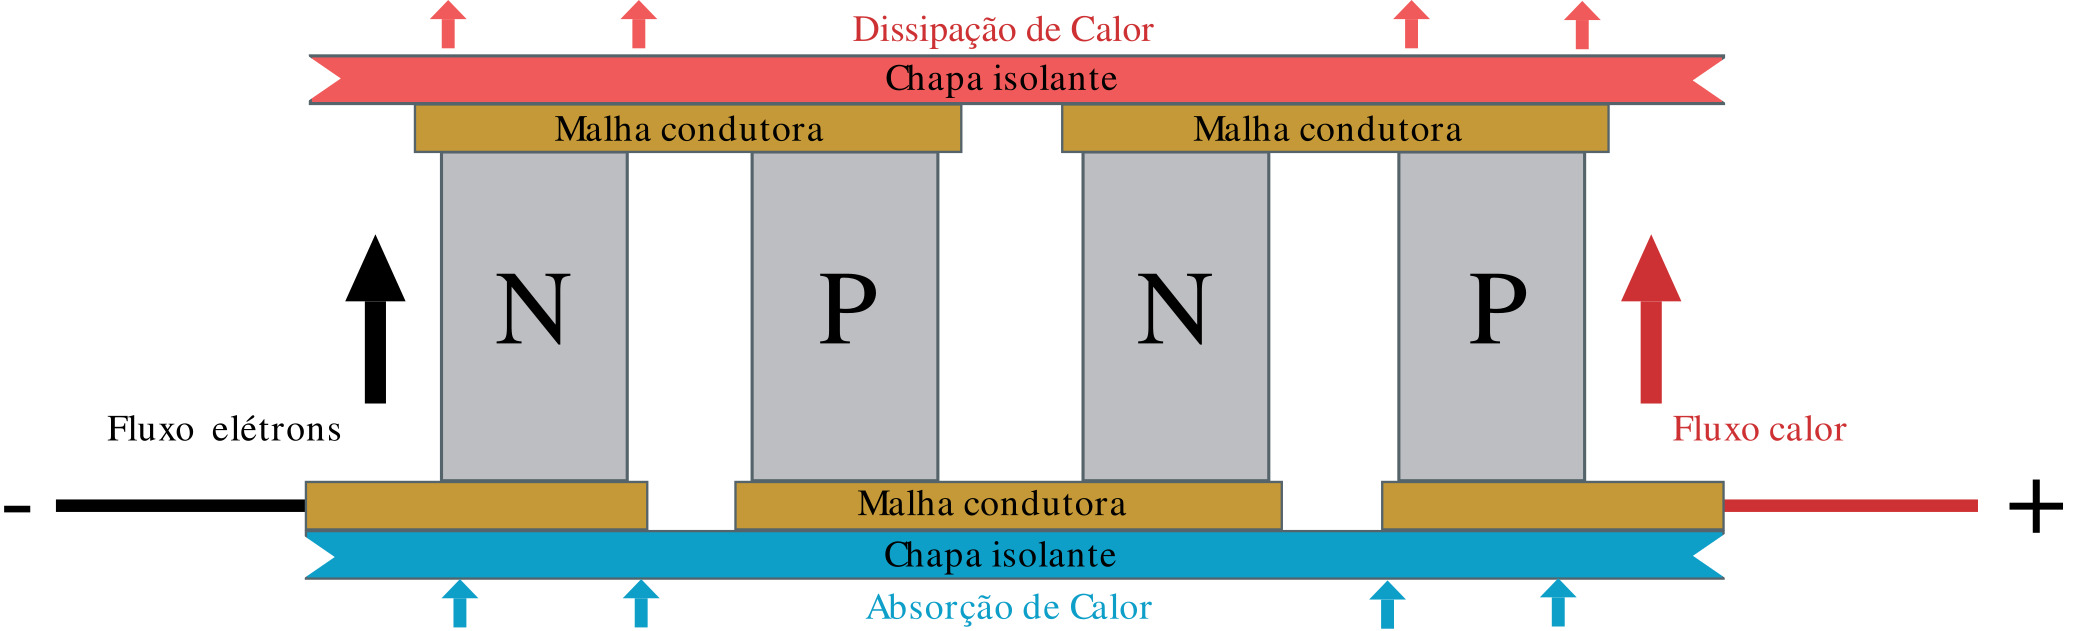
\includegraphics[scale=.8]{Esquema_Pastilha_de_Peltier.jpg}
		\caption{Funcionamento do Efeito Peltier}
		\label{peltier}
	\end{figure}
	
	\noindent A energia térmica do sistema é proporcional à corrente elétrica que percorre o sistema, sendo possível assim definir o calor associado pelo efeito pela Equação \ref{peltier_eq}.
	
	\begin{equation}
	Q_{p} = \Pi \cdot I
	\label{peltier_eq}
	\end{equation}
	
	\noindent Onde $Q_{p}$ é o calor associado, $\Pi$ o coeficiente de Peltier, e $I$ a corrente elétrica gerada pelo sistema. O coeficiente de Peltier esta relacionado com o coeficiente de Seebeck pela Equação \ref{peltier_eq2} e pela Equação \ref{peltier_eq3}.
	
	\begin{equation}
	\Pi = T \frac{S}{q}
	\label{peltier_eq2}
	\end{equation}
	
	\begin{equation}
	Q_{p} = S \cdot I \cdot T
	\label{peltier_eq3}
	\end{equation}
	
	\section{Efeito Thompson}
	
	O efeito Thompson, descreve a capacidade de uma corrente elétrica passando em um material no qual existe um gradiente de temperatura leva à produção de calor neste material, que atua em conjunto com o Efeito Joule, temos na Equação \ref{thompson_eq} o calor produzido por unidade de volume gerado por uma densidade de corrente $\overrightarrow{J}$.
	
	\begin{equation}
	Q = \rho J^{2} - \mu_{Th}\overrightarrow{J}\cdot \nabla_{r}T
	\label{thompson_eq}
	\end{equation}
	
	\noindent Onde $\rho$ é a resistividade do condutor e $\mu_{Th}$ o coeficiente de Thompson, podemos identificar a componente do Efeito Joule descrito por $\rho J^{2}$ e o segundo termo, o efeito Thompson que muda de sinal dependendo da direção de $\overrightarrow{J}$ sendo descritos como efeito positivo/negativo de Thompson para cada situação. E também vale ressaltar que o coeficiente de Thompson esta relacionado com o coeficiente termo-elétrico(S) pela Equação \ref{thompson_eq2}.
	
	\begin{equation}
	S = q \int_{0}^{T} \frac{\mu_{Th}}{T} \mathrm{d}T
	\label{thompson_eq2}
	\end{equation}
	
		\section{Potência Termoelétrica}
	
	A potência termoelétrica é a relação que expressa a quantidade de milivolts, gerada a cada variação de $1^\degree C$ de variação de temperatura, expressa na Equação \ref{potencia_termoeletrica}.
	
	\begin{equation}
	P_{T} = \frac{mV}{^{\circ}C}
	\label{potencia_termoeletrica}
	\end{equation}
	
	\singlespacing
	
	Como a tensão gerada por $1^{\circ}C$ de variação é um número muito pequeno e como a variação da F.E.M. gerada em função da temperatura não é linear, é usual definir-se a potência termoelétrica média no intervalo de utilização de cada termopar e multiplicar-se este valor por 100\degree C.
	
	\singlespacing
	
	A potência termelétrica é muito útil na caracterização e comparação dos termopares, indicando principalmente a sensibilidade do dispositivo. Quanto maior for a sua variação de tensão, mais sensível é o sensor.
	
	\newpage
	\section{Leis Termoelétricas}
	
	Com a descoberta dos efeitos termoelétricos, a partir da aplicação das leis da termodinâmica, foi enunciado as três leis que contêm toda a base da teoria termoelétrica, aplicados em componentes como termopares. E Portanto a partir destas leis, podemos compreender todos os fenômenos que ocorrem na medida de temperatura com estes sensores. 
	
	\subsection{Lei do circuito Homogêneo}
	
	A lei do circuito homogêneo enuncia que: “A F.E.M. termal, desenvolvida em um circuito termoelétrico de dois metais diferentes, com suas junções às temperaturas T1 e T2, é independente do gradiente de temperatura e de sua distribuição ao longo dos fios." Isso significa que, a F.E.M. medida depende única e exclusivamente da composição química dos dois metais e das temperaturas existentes nas junções.
	
	\singlespacing
	
	Um exemplo de aplicação prática desta lei é que podemos ter uma grande variação de temperatura em um ponto qualquer, ao longo dos fios dos Termopares, como esquematizado na Figura \ref{lei1}, que esta não influirá na F.E.M. produzida pela diferença de temperatura entre as juntas. Portanto, garante-se fazer medidas de temperatura em pontos bem definidos com os Termopares, pois o importante é a diferença de temperatura entre as juntas.
	
	\singlespacing
	
	\begin{figure}[htbp]
		\centering
		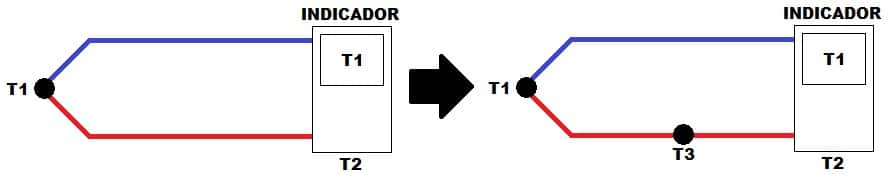
\includegraphics[scale=.4]{Lei1.jpg}
		\caption{Exemplo da Lei do Circuito Homogêneo}
		\label{lei1}
	\end{figure}
	
	\subsection{Lei dos Metais Intermediários}
	
	A lei dos metais intermediários enuncia que: "A soma algébrica das F.E.M. termais, em um circuito composto de um número qualquer de metais diferentes, é zero se todo o circuito estiver à mesma temperatura”. Em outras palavras, esta lei estabelece que em um circuito, composto de dois metais diferentes, a tensão gerada não será modificada caso seja inserido um outro metal intermediário em qualquer ponto do circuito, desde que as junções recém formadas sejam mantidas a uma mesma temperatura devida. Isto ocorre devido ao fato de que a tensão gerada a partir destas duas novas junções será igual a zero. Este princípio por sua vez garante o uso de fios de extensão, bem como de conectores, como  representado na Figura \ref{lei2}.
	
	\singlespacing
	
	\begin{figure}[htbp]
		\centering
		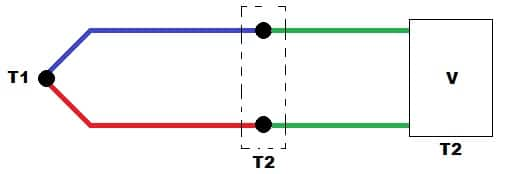
\includegraphics[scale=.5]{lei2.jpg}
		\caption{Exemplo dos Metais Intermediários}
		\label{lei2}
	\end{figure}
	
	\newpage
	\subsection{Lei das Temperaturas Intermediárias}
	
	“A F.E.M. produzida em circuito termoelétrico de dois metais homogêneos e diferentes entre si, com as suas junções às temperaturas T1 e T3 respectivamente, é a soma algébrica da F.E.M. deste circuito, com as junções às temperaturas T1 e T2, e a F.E.M. deste mesmo circuito, com as junções às temperaturas T2 e T3”. Podemos ver os esquema dessa lei representada na Figura \ref{lei3}.
	
	\singlespacing
	
	Assim, como consequência direta deste princípio, pode-se efetuar correções caso termopares que foram calibrados a uma determinada temperatura de referência possam ser utilizados em qualquer outra temperatura de referência.
	
	\begin{figure}[htbp]
		\centering
		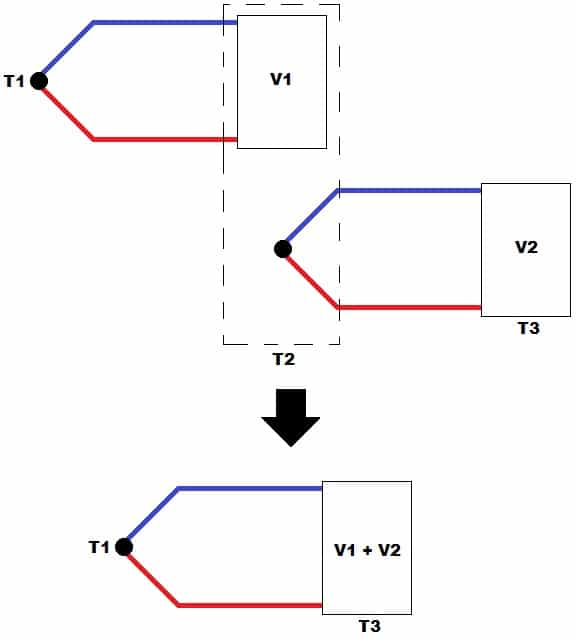
\includegraphics[scale=.4]{lei3.jpg}
		\caption{Exemplo das Temperaturas Intermediárias}
		\label{lei3}
	\end{figure}
	
	\chapter{Aplicações}
	
	Termopares podem ser utilizados em equipamentos via medição de tensão, geralmente utilizando algum aspecto de instrumentação eletrônica. A partir da tensão mensurada, é possível calcular a temperatura utilizando métodos de \textit{look-up table} e interpolação. Com uma interpolação combinando métodos de segundo e terceiro é possível ter um erro mínimo para um bom \textit{range} de temperatura. 
	
	É possível, ainda, comprar designs analógicos e digitais de referência para instrumentação de termopares. Um exemplo é o design \texttt{TIDA-00468} da \textit{Texas Instruments\textsuperscript{TM}}, que oferece sensoriamento de -270\degree C até +1372\degree C para termopares do tipo K.
	
	\begin{figure}[H]
		\centering
		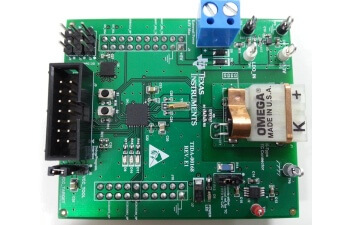
\includegraphics[scale=0.6]{tida.jpg}\\
		\caption{Placa \textit{front-end} \texttt{TIDA-00468}, contendo sistema digital e filtros para termopares do tipo K. Fonte: Texas Instruments.}
	\end{figure}
	
	A escolha do design é importante, visto que o custo agregado ao sensoriamento pode ser até maior que o custo do dispositivo em si, apesar do sensoriamento digital ser relativamente barato no presente momento.
	
	Outras aplicações de termopares incluem transformação de energia térmica em energia elétrica. Um bom exemplo disso são \textbf{RITEG}s, \textit{Radioisotope Thermoelectric Generators}. Tais dispositivos são utilizados em diversos satélites e em missões espaciais. 
	
	O sistema consiste em um material radiotivo, que gera calor via decaimento $\alpha, \beta$ ou $\gamma$ de um núcleo radioativo (por exemplo, um cilindro de \texttt{plutônio-238}) com diversos termopares ao redor, com seus lados "frios" respectivamente grudados em aletas.
	
	\begin{figure}[H]
		\centering
		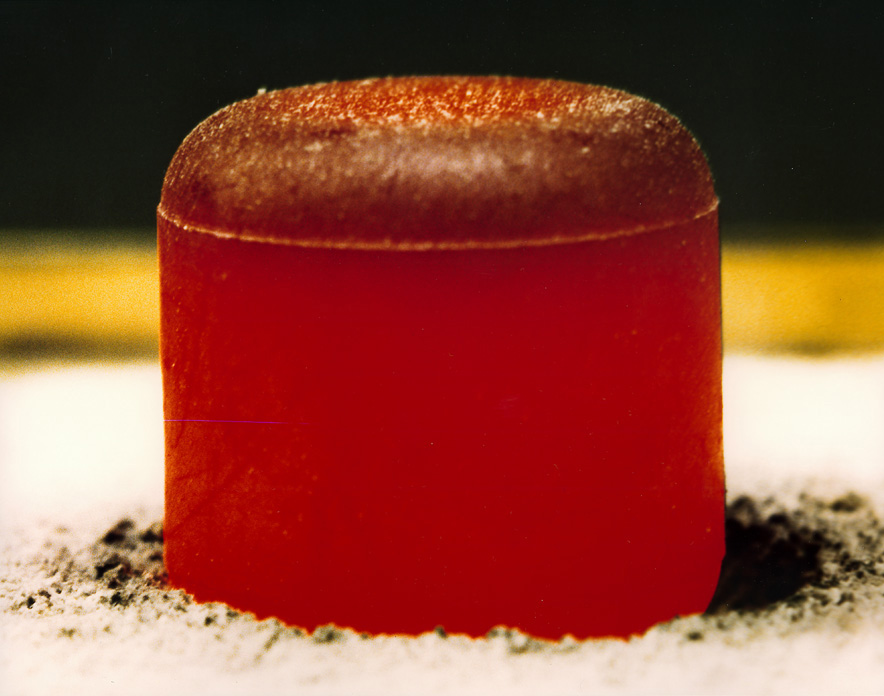
\includegraphics[scale=0.06]{plutonium_pellet.jpg}\\
		\caption{Pellet de Plutônio-238 do RTG da Curiosty Rover. Produz cerca de $110$W.\\ Fonte: Idaho National Laboratory CC-by-2.0.}
	\end{figure}

	Os termopares utilizados nesse caso específico das missões de telescópio são de silício-germânio (SiGe), e foram escolhidos para essa aplicação por apresentarem bom comportamento na \textit{range} de temperatura de trabalho e uma boa resistência mecânica, novamente enfatizando que a escolha de termopares vai muito além de alguns poucos parâmetros.
\newpage
	O esquema geral pode ser apresentado pelo seguinte esquemático:
	
	\begin{figure}[H]
		\centering
		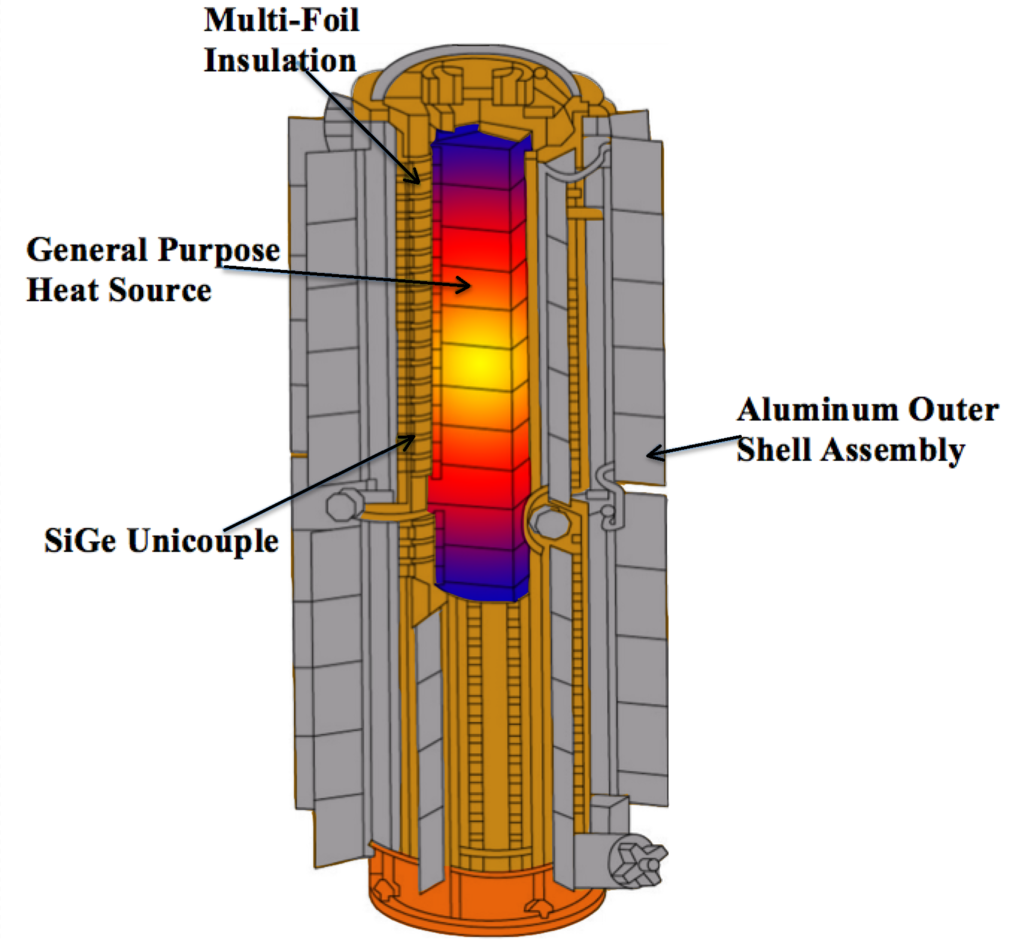
\includegraphics[scale=0.4]{sige_rtg.png}\\
		\caption{Esquemático de um RITEG. Fonte: Parker Beatty CC BY-SA 4.0.}
	\end{figure}

	O princípio de conversão de energia é explicado pelo já citado efeito \textit{Seeback} (ver seção 2.1). 
	
	Equipamentos desse tipo foram usados nas missões do programa Apollo, e um exemplo desse equipamento (em cinza, no centro) pode ser observado na seguinte fotografia tirada na Lua (outros módulos de outras missões que retornaram com os astronautas ainda se encontram no fundo do mar).
	
	Informações exatas quantificando a produção de energia por esses dispositivos são, no entanto, escassas.
	
		\begin{figure}[H]
		\centering
		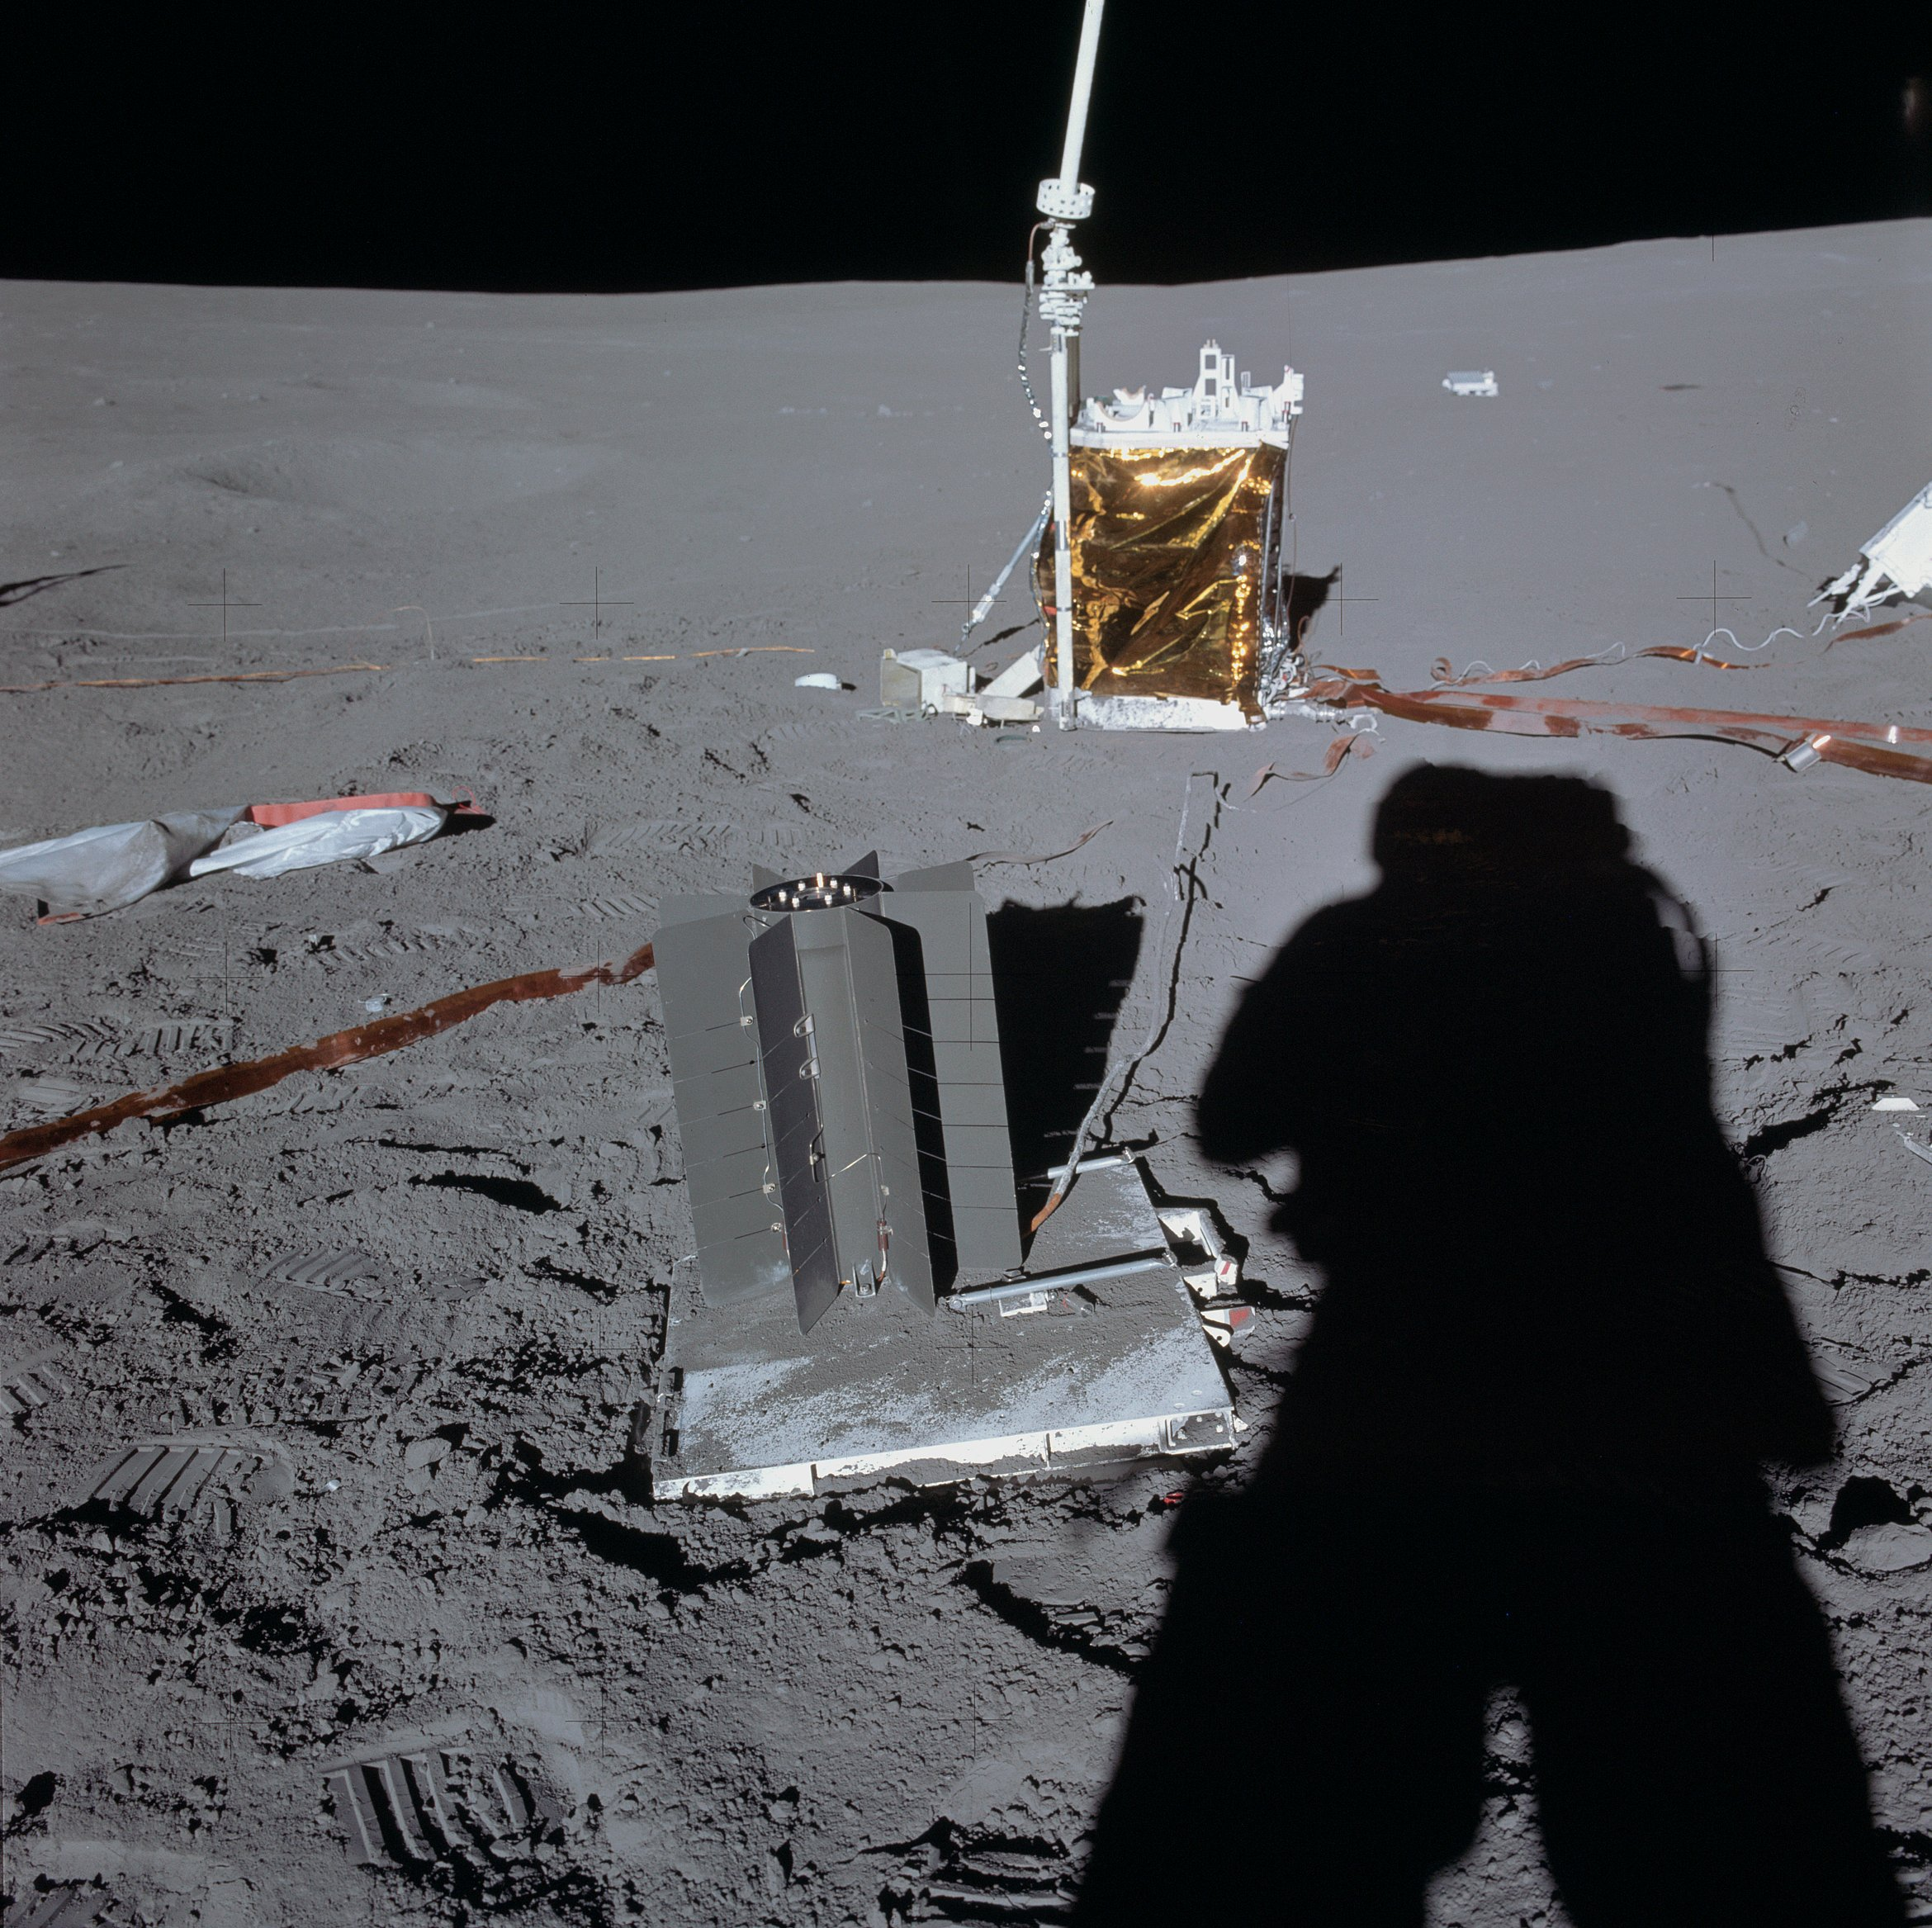
\includegraphics[scale=0.7]{apollo.jpg}\\
		\caption{Um RITEG na Lua. Fonte: NASA/Alan Shepard PD-USGOV-NASA.}
	\end{figure}

	
	
	\begin{landscape}
			A seguinte tabela sumariza alguns - mas não todos - tipos de termopares comerciais e suas características físicas de acordo com [REFERÊNCIA]. Vale notar que essa tabela não leva em consideração, por exemplo, características mecânicas dos dispositivos, ou resistência a interferência eletromagnética.
			
			\vspace{2cm}
			
		\begin{center}
			\begin{tabular}{|c|c|c|c|c|c|}
				\hline 
				Type & Positive Material	 & Negative Material	 & Accuracy\footnote{De acordo com a Comissão Eletrotécnica Internacional 584-2}
				Class 2	 & Range \degree C
				(extension) \\ 
				\hline 
				B  & Pt, 30\%Rh	        & Pt, 6\% Rh                          & 0.5\% 800\degree C     & 50 to 1820 \\ 
				\hline 
				E  & Ni, 10\%Cr	        & Cu, 45\% Ni	                      & 0.5\% or 1.7\degree C  & -270 to 1000 \\ 
				\hline 
				J  & Fe                 & Cu, 45\% Ni	           			  & 0.75\% or 2.2\degree C & -210 to 1200 \\ 
				\hline 
				K  & Ni, 10\%Cr         & Ni, 2\% Al 2\% Mn 1\% Si            & 0.75\% or 2.2\degree C & -270 to 1372 \\ 
				\hline 
				N  & Ni, 14\%Cr 1.5\%Si & Ni, 4.5 \% Si 0.1\% Mg              & 0.75\% or 2.2\degree C & -270 to 1300 \\ 
				\hline 
				R  & Pt, 13\%Rh         & Pt                                  & 0.25\% or 1.5\degree C & -50 to 1768 \\ 
				\hline 
				S  & Pt, 10\%Rh	        & Pt                                  & 0.25\% or 1.5\degree C & -50 to 1768 \\ 
				\hline 
				T  & Cu                 & Cu, 45\% Ni                         & 0.75\% or 1.0\degree C & -270 to 400 \\ 
				\hline 
			\end{tabular} 
		\vspace{0.5cm}
		
		\footnotesize{Tabela 2.3.1. Fonte: National Institute of Standards and Technology.}
		\end{center}
	\end{landscape}
	Esses dispositivos também podem ser classificados em dois grupos principais:
	
	\begin{itemize}
		\item Nobres: Contém ligas nobres na sua composição, como platina. Geralmente possuem uma temperatura mais alta de operaçã. Exemplos incluem os tipos R, S e B.
		\item Base: Mais comuns, geralmente feitos com ligas de níquel em um ou ambos materiais. Exemplos incluem os tipos J, K, T e E. O nome "base" vem do inglês "\textit{base metal}", denotando um metal relativamente barato, oposto aos metais preciosos.
	\end{itemize}
	
	\subsection{Construção}
	
	Tipos de termopares diferentes servem propósitos diferentes. Dentro dos tipos de junções, existem características de operação, e além disso, existem formas de construção que podem ser melhor utilizadas em algum ambientes específico. Questões como vibrações mecânicas, radiação ou operação Ininterrupta são considerações que devem ser realizadas ao escolher o tipo de termopar, e o próprio meio de instrumentação.
	
	Quatro tipos de construção do dispositivo em si podem ser encontradas:
	
	\begin{itemize}
		\item Aterrados: Os dois materiais são soldados juntamente com o invólucro. Permite respostas relativamente rápidas, porém pode apresentar um mau desempenho em aplicações com muita interferência eletromagnética.
		
		\item Não aterrados comum: Os dois materiais são isolados do invólucro por algum tipo de material. Mais estável que o Aterrado, porém tem um tempo de resposta significativamente mais lento.
		
		\item Expostos: A junção é totalmente exposta, sem invólucro. Melhor tempo de resposta, porém é extremamente susceptível a corrosão.
	\end{itemize}

	\section{Simulações}
	Argumentavelmente uma das melhores ferramentas disponíveis para o engenheiro é a simulação via computador, levando a questão de possibilidade de simulação de dispositivos termopares.
	
	Órgãos como a ABNT fazem estudos extensivos de caracterização de termopares em condições específicas, e é também possível encontrar dados sobre os diferentes dispositivos de fabricantes comerciais privados.
	
	Na tabela seguinte, é possível observar alguns valores de temperatura versus EMF de um certo termopar, calculados pela ABNT.
	
	\begin{figure}[H]
		\centering
		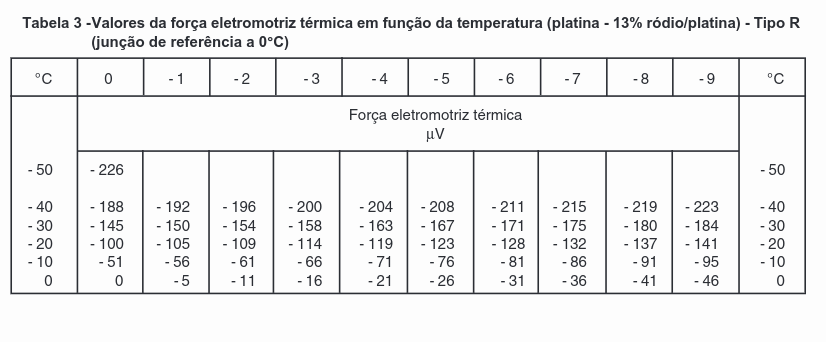
\includegraphics[scale=0.5]{abnttable.png}\\
		\caption{Tabela de EMF versus Temperatura para um termopar tipo R. Fonte: ABNT NBR 12771:1999.}
	\end{figure}

	É possível então empregar métodos matemáticos, afim de se aproximar o comportamento de cada dispositivo. O mais prático parece ser usar uma expansão polinomial de grau suficiente de forma a aproximar a curva de temperatura vs. EMF, seja com métodos como splines, aproximações integrais etc.

	De forma que a tensão $\mathfrak{E}$ pode ser representada por
	
	\[\mathfrak{E}_{ref} = c_{0} + \sum_{k = 1}^{N}c_{i} \cdot t^{i}\]
	
	A ABNT - e outros órgãos, como o NIST - já cedem os coeficientes $c_{i}$, facilitando e ajudando no processo de homogenização de empresas que compram esses certificados.
	
		\begin{figure}[H]
		\centering
		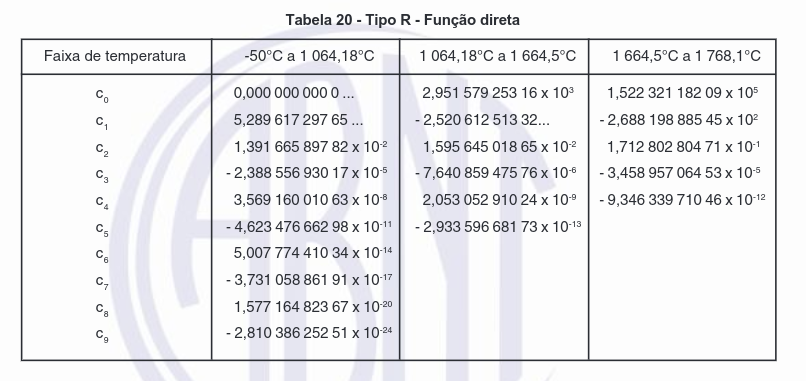
\includegraphics[scale=0.5]{abntcoeffs.png}\\
		\caption{Coeficientes polinomiais para um termopar tipo R. Fonte: ABNT NBR 12771:1999.}
	\end{figure}

	Dessa forma, é possível uniformizar e assegurar a qualidade de termopares fabricados sob normação, dado que a empresa que produz o produto pode criar sua própria tabela de temperatura vs EMF, derivar uma aproximação polinomial no intervalo desejado do tipo
	
	\[\mathfrak{E}_{mes} = a_{0} + \sum_{k = 1}^{N}a_{i} \cdot t^{i}\]
	
	e utilizar uma métrica de tolerância como
	
	\[\|\mathfrak{E}_{ref} - \mathfrak{E}_{mes}|\] 
	
	Também é possível utilizar um método como Newton-Raphson afim de obter a temperatura dado uma EMF medida, o que exige uma função de calibração que também pode ser encontrada em documentos da natureza da ABNT NBR 12771:1999.
	
	Os seguintes gráficos foram gerados e adaptadas usando a biblioteca \texttt{thermocouples\_reference}, que funciona com um envelope ao redor das curvas normadas de temperatura vs EMF da NIST, OMEGA e ASTM. É claro que possuímos um ambiente inerentemente discreto no computador digital, porém com boas referências de medidas reais, tomadas com rigidez e método científico, é possível obter resultados extremamente precisos por interpolação, com tolerâncias tão pequenas quanto quisermos.

	\begin{figure}[htbp]
	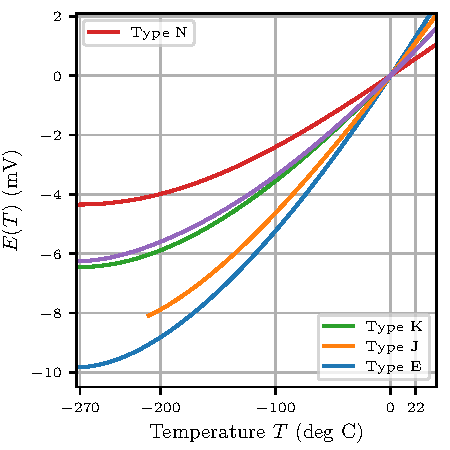
\includegraphics[scale=1]{src/lowTerm.pdf}
	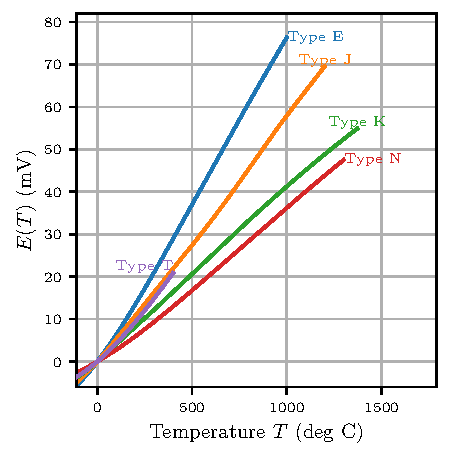
\includegraphics[scale=1]{src/medTerm.pdf}
	\begin{center}
		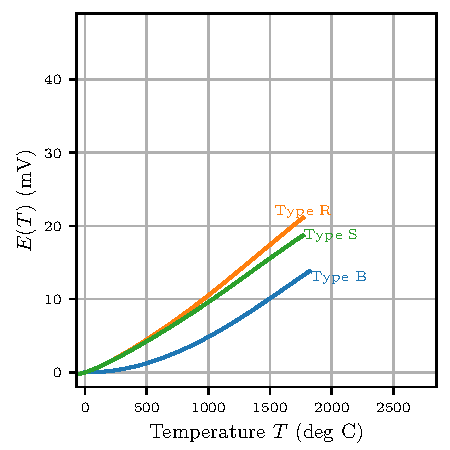
\includegraphics[scale=1]{src/highTerm.pdf}
		
		\caption{Gráficos de temperaturas vs EMF dos termopares citados na tabela 2.3.1. Fonte: Os autores utilizando biblioteca supracitada, com dados dos órgãos supracitados.}
	\end{center}
	\end{figure}

\newpage

	\chapter{Conclusão}
	O estudo realizado demonstra que a classificação de termopares não é feita de forma binária, com peculiaridades em cada aplicação: tempo de resposta, faixa de temperatura, precisão e outras características supracitadas. Esses aspectos devem ser levados em consideração na hora de se escolher o tipo de termopar a ser usado para correta aferição de temperatura, ou seja, o melhor termopar é aquele que melhor se adequa a sua aplicação. 
	
	Vale contar, também, que o termopar é muito mais do que um dispositivo \textit{standalone}, e sim um transdutor que compõe parte de um sistema integral, numa junção multidisciplinar de física teórica, processamento e condicionamento de sinais, como observado em produtos comerciais especializados para tal.
	
	O esclarecimento dos processos que ocorrem, como o efeito Seebeck e o efeito Peltier nos permitem compreender o funcionamento desse dispositivo, e, de fato, como simular, tomar nota sobre seu comportamento e limitações.
	
	% \section{Referências}
	\nocite{*}
	

	\bibliography{IEEEabrv,materiais}
	\bibliographystyle{IEEEtran}
	
\end{document}


